\section{Normalización y normalización por lotes}

Un factor importante a tomar en cuenta para un buen desempeño del entrenamiento son las magnitudes del datos de entrada a la red. Entonces para mejorar el desempeño del algoritmo de optimización nos conviene pre-procesar los datos de entrada. Esto mediante una técnica que se llama normalización (\emph{normalization} en inglés).

La técnica que hemos utilizado son técnicas de optimización basadas en el gradiente, la cual a una función de error se calcula el gradiente, este nos da la dirección del máximo descenso, para  hacer aproximaciones discretas en los parámetros hasta que tratemos de llegar al mínimo de la función.
 
Para poder realizar lo anterior necesitamo que las magnitudes de los datos de entrada no esten muy dispersas, es decir que no nos encontremos con situaciones donde estemos manejando decimales para unos datos y para otros unidades de millones. En estos casos la función de error nunca va a terminar de ajustarse correctamente a estos datos, pues en ocaciónes los parametros para ajustar, van a avanzar de forma distorsionada. Dando la impresión que para unos datos el gradiente avanza muy rapido al centro, mientras que para otros datos avanza muy lento, esto porque vamos a tener curvas de nivel demasiado elípticas (ver la figura \ref{fig:curvasNivel}), entonces al tomar la dirección que nos de el gradiente, nos va a mover desplazar muy violentamente en algunas y muy lento para otras. Cuando se intente hacer descenso por el gradiente en estas regiones lo que va a pasar es que el vector va a oscilar muy violentamente y  nos va a dificultar mucho llegar al minimo.

Por el contrario, si las magnitudes con las que trabajamos son del mismo orden y contribuyen numéricamente de una manera más proporcionada al error, entonces vamos a tener curvas de nivel  más circulares (ver la figura \ref{fig:curvasNivel}). Cuando calculemos el gradiente, la perpendicular se aproximará durante más tiempo a la dirección de máximo descenso. 

\begin{figure}[H]
 \centering
 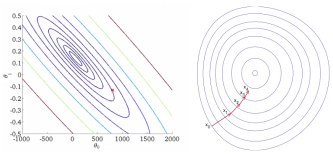
\includegraphics[scale=0.5]{../Figuras/curvasDeNivel.png}
 \caption{Izq: J la función de error con alta excentricidad. Der: J con curvas de nivel tendiendo a círculos}
 \label{fig:curvasNivel}
\end{figure}

Entonces para asegurar un buen desenso por el grandiente, vamos a preferir siempre trabajar con curvas de nivel circulares, para esto vamos a usar la normalización.

La normalización conciste en centrar los datos aproximadamente en el intervalo $[-1.0, 1.0]$, este intervalo no es estricto para todas las redes basta con definir las magnitudes en un intervalo aceptable para tener curvas de nivel circulares. 

Existen varias fórmulas para realizar la normalización, se sugiere la siguiente forma:
\begin{itemize}
 \item Calcular \emph{la media} $\mu_i$ y \emph{varianza} $\sigma_{i}^2$ para cada característica $i$ en los datos del conjunto de entrenamiento $X$.
 \begin{itemize}
  \item Las formulas son las siguientes, con $X_i$ la columna con la i-ésima característica en los datos de entrenamiento $X$.\\
  \begin{equation}
   \mu_{i} = \dfrac{1}{m}\sum_{i=1}^{m}x_{i} 
  \end{equation}
  \begin{equation}
   \sigma_{i}^{2} = \dfrac{1}{m}\sum_{i=1}^{m}(x_{i}-\mu)^2 
  \end{equation}
  \begin{equation}
   X_{i} = \dfrac{X_{i}-\mu}{\sigma^{2}}
  \label{eq:tres}
  \end{equation}
 \end{itemize}
    \item La media es el promedio de los datos de entrada.
    \item La varianza es una medida de dispersión, para ver que tan separados estan los datos unos de otros.
    \item La reasignación para cada $X_i$ va a ser, la resta $X_i -\mu$, que va a centrar los datos alrededor del cero, y la división por la varianza $\sigma^2$ que va a encoger los intervalos de distancia entre los datos. 
\end{itemize}

 
\begin{itemize}
 \item Una vez que la red se entreno con datos normalizados, \textit{es necesario almacenar las medias y varianzas} utilizadas durante el entrenamiento con el conjunto de entrenamiento $X$.
 \item Estos valores serán utilizados para normalizar datos nuevos que vayan a ser evaluados en la red. Esto para evitar que los nuevos datos usen magnitudes fuera del intervalo usado durante el entrenamiento de la red.
\end{itemize}

\begin{definition}
 \emph{La normalización} permite reducir la excentricidad en la función de error provocada por la disparidad entre los datos de entrada.
\end{definition}
  
 Entonces ya tenemos resuelta la situación de la disparides entre los datos de entrada. Ahora tenemos que, al calcular los valores para las capas intermedias, los valores pueden cambiar sus rangos para las neuronas intermedias. Para esta situación tenemos la normalización por lotes (\emph{bach normalization} en inglés).
 
La normalización por lotes aplica los beneficios de la normalización a las capas intermedias, haciendo que estás den valores en intervalos no muy grandes para las siguientes capas.

Una ventaja que nos da esta herramienta es que los algoritmos de optimización podrán utilizar \textit{tazas de aprendizaje más altas}, porque los brincos discretos del algoritmo no cambiarán drásticamente el comportamiento de la función de error durante un intervalo más largo.

Otra ventaja es que al normalizar entre capas, permite que cada capa calcule características distintas, independientemente que se otorguen ejemplares con mucho sesgo en una característica en especial. Permitiendo una mejor clasificación aún con datos nuevos. 

\begin{definition}
 La \emph{normalización por lotes} conciste en: 
 \begin{enumerate}
  \item  Normalizar la salida de la capa de activación anterior restando su media y dividiendo entre la desviación estándar.
  \item Hacer descenso por el gradiente estocástico.
  \item Dos paremetros: $\gamma$ una desviación estandar y $beta$ una media para corrimiento.
 \end{enumerate}
\end{definition}

Cuando se use el descenso por el gradiente estocástico (el descenso por el gradiente por lotes) modificará los pesos para optimizar $J$ la función de error, y probablemente contrarreste el efecto de la normalización.
Para evitarlo, se añaden dos parámetros, también entrenables: $\gamma$ una desviación estándar y $\beta$ una media para corrimiento, la idea es que el algoritmo tienda a
modificar estos dos para ese fin, en lugar de los pesos, de modo que los pesos produzcan un cómputo más estable.

Entonces la idea concreta es que dado un $B$ el minilote con $x_i$ sus ejemplares, las entradas $y_i$ para la capa siguiente se
calculan con las formulas:
  \begin{equation}
   \mu_{B} = \dfrac{1}{m}\sum_{i=1}^{m}x_{i} 
  \end{equation}
  \begin{equation}
   \sigma_{B}^{2} = \dfrac{1}{m}\sum_{i=1}^{m}(x_{i}-\mu_{B})^2 
  \end{equation}
  \begin{equation}
   x_{i} = \dfrac{X_{i}-\mu_{B}}{ \surd \sigma_{B}^{2} + \varepsilon}
  \label{eq:tres}
  \end{equation}
  \begin{equation}
   y_{i} = \gamma x_{i}+\beta \equiv BN_{\gamma,\beta}(x_{i})
  \label{eq:tres}
  \end{equation}

con $\varepsilon$ una constante agregada para mantener la estabilidad numérica.
